\tikzsetnextfilename{forward_table}
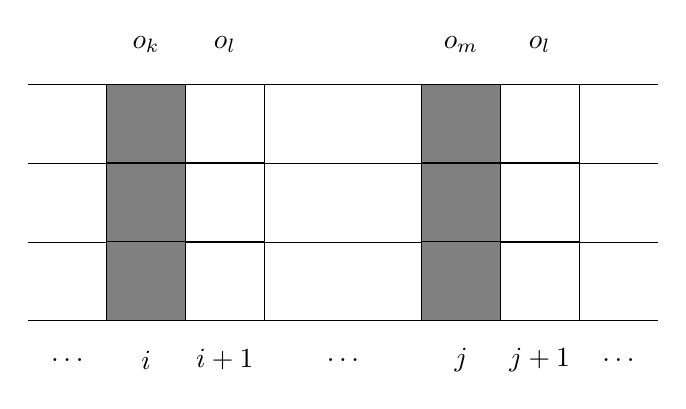
\begin{tikzpicture}
  \tikzstyle{box} = [draw=black, minimum width=10mm, minimum height=10mm];
  \tikzstyle{gray_box}  = [box, fill=gray];
  \tikzstyle{white_box} = [box];


  \draw[very thin] (-1.5, -0.5) -- (6.5, -0.5);
  \draw[very thin] (-1.5, 0.5)  -- (6.5, 0.5);
  \draw[very thin] (-1.5, 1.5)  -- (6.5, 1.5);
  \draw[very thin] (-1.5, 2.5)  -- (6.5, 2.5);

  \node[gray_box]  at (0, 0) {};
  \node[white_box] at (1, 0) {};
  \node[gray_box]  at (4, 0) {};
  \node[white_box] at (5, 0) {};

  \node[gray_box]  at (0, 1) {};
  \node[white_box] at (1, 1) {};
  \node[gray_box]  at (4, 1) {};
  \node[white_box] at (5, 1) {};

  \node[gray_box]  at (0, 2) {};
  \node[white_box] at (1, 2) {};
  \node[gray_box]  at (4, 2) {};
  \node[white_box] at (5, 2) {};

  \node at (0, 3) {$o_k$};
  \node at (1, 3) {$o_l$};
  \node at (4, 3) {$o_m$};
  \node at (5, 3) {$o_l$};

  \node at (-1, -1) { $\dots$};
  \node at (0, -1)  { $i$};
  \node at (1, -1)  { $i+1$};
  \node at (2.5, -1)  { $\dots$};
  \node at (4, -1)  { $j$};
  \node at (5, -1)  { $j+1$};
  \node at (6, -1)  { $\dots$};
\end{tikzpicture}
%%% Local Variables:
%%% mode: latex
%%% TeX-master: "../master"
%%% End:
